
\documentclass[../relatorio.tex]{subfiles}
\begin{document}
De forma a ilustrar alguns dos diagramas de sequência desenvolvidos, foram escolhidos 3 use cases com o objetivo de 
apresentar todos os diagramas referentes a estes e também qual foi a estratégia escolhida para os resolver.
Foram considerados 3 \textit{uses cases} "principais", nomeadamente o Fazer Orçamento, o Realizar Reparação e ainda o
Pedir Reparação Expresso.

\subsection{Fazer Orçamento}
Tal como é referido no use case, quando o técnico pretende fazer um orçamento, este solicita o pedido de orçamento mais 
antigo. O sistema para responder a este pedido, constroi um Set ordenado por ordem descrescente da data de criação com todos os Orçamentos 
em que o estado é "porCalcular". Set este construído a partir do método getOrcamentosAtivos(), chamado pelo getOrcamentoMaisAntigo() que lhe retira
o primeiro elemento.
\begin{figure}[!ht]
    \centering
    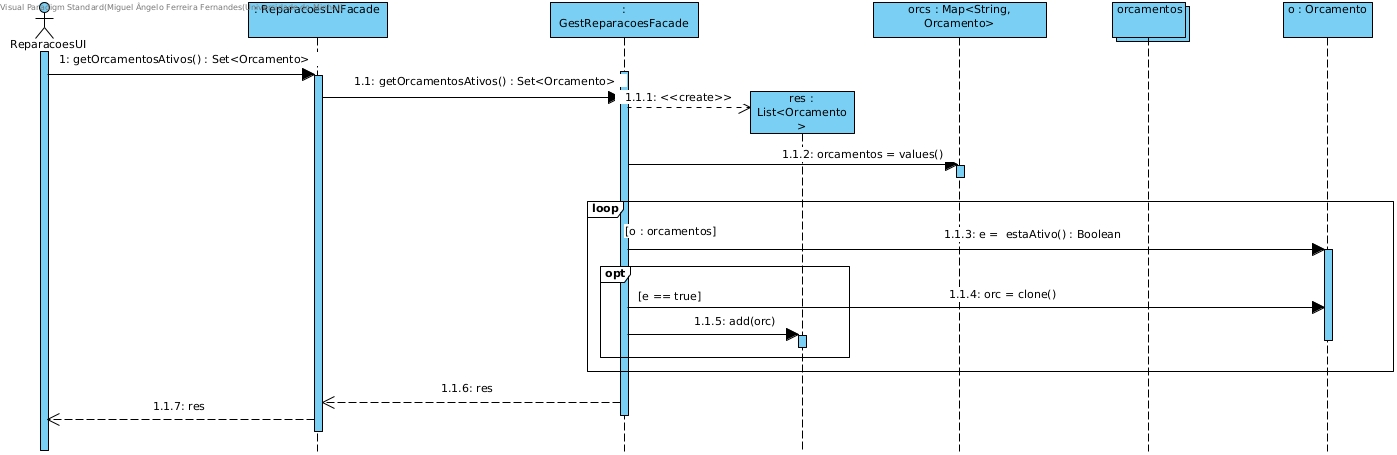
\includegraphics[scale=0.30]{../assets/diagramas_sequencia/sd-GetOrcamentosAtivos.jpg}
    \caption{Diagrama de sequência getOrcamentosAtivos}
\end{figure}

Depois de saber qual o Orçamento que tem de calcular, o técnico analisa o equipamento e vai construindo o plano de trabalhos adicionando 
sequencialmente os passos necessários para a sua reparação. Cada passo é identificado por um nome e é caracterizado pelo tempo estimado e ainda
por o material que é expectável usar.

\begin{figure}[!ht]
    \centering
    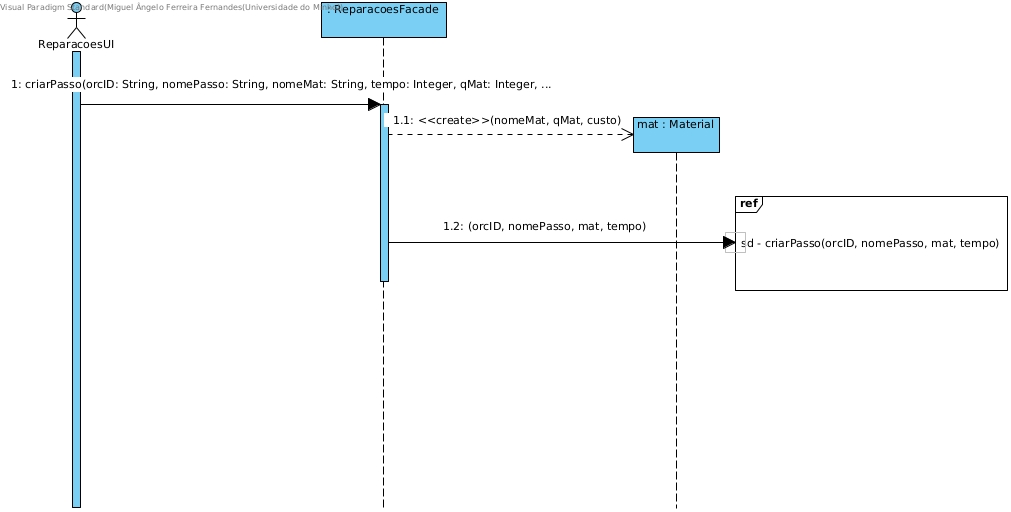
\includegraphics[scale=0.35]{../assets/diagramas_sequencia/sd-criarPasso1.jpg}
    \caption{Diagrama de sequência criarPasso(1)}
\end{figure}

\begin{figure}[!ht]
    \centering
    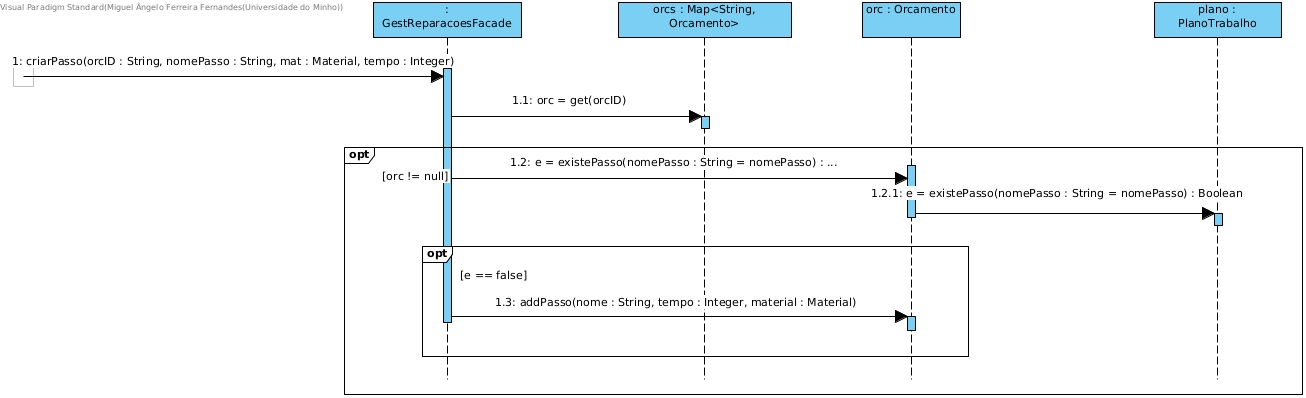
\includegraphics[scale=0.30]{../assets/diagramas_sequencia/sd-criarPasso2.jpg}
    \caption{Diagrama de sequência criarPasso(2)}
\end{figure}

Quando todos os passos já foram adicionados e o plano de trabalhos já foi concluído o técnico pode gerar o Orçamento e registar o 
envio do mesmo ao cliente. O estado do orçamento muda de "porCalcular" para enviado e é adicionado às comunicações do Orçamento o 
contacto referente ao envio.

\begin{figure}[!ht]
    \centering
    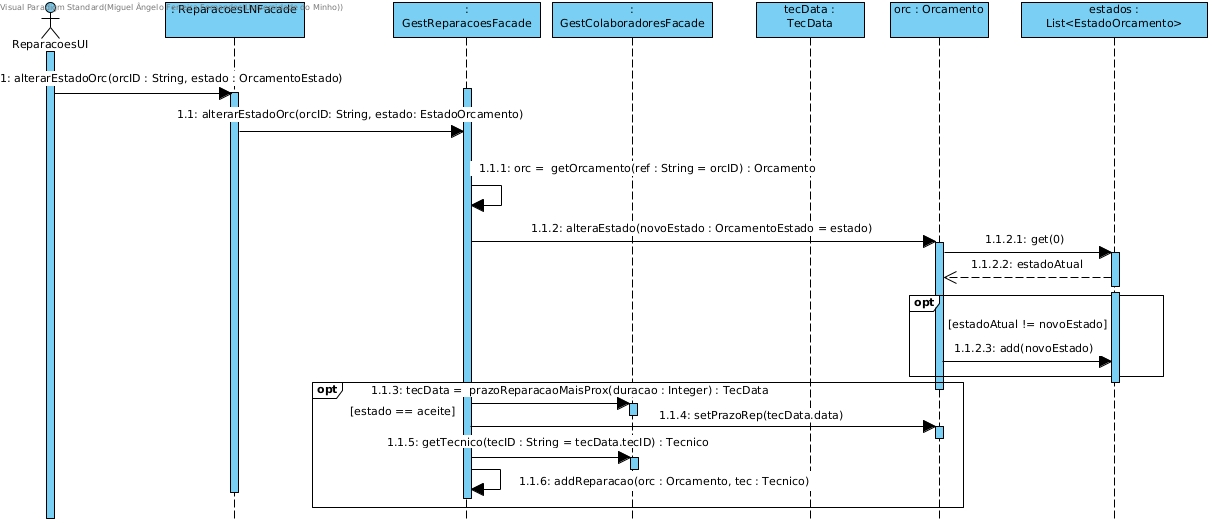
\includegraphics[scale=0.30]{../assets/diagramas_sequencia/sd-alterarEstadoOrc.jpg}
    \caption{Diagrama de sequência alterarEstadoOrc}
\end{figure}

\begin{figure}[!ht]
    \centering
    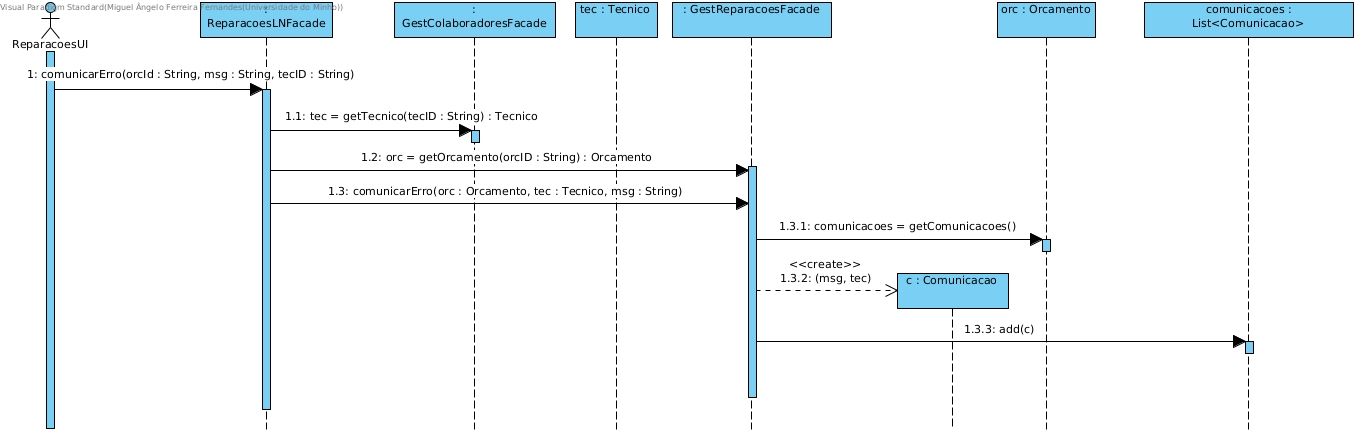
\includegraphics[scale=0.30]{../assets/diagramas_sequencia/sd-ComunicarErro.jpg}
    \caption{Diagrama de sequência comunicarErro}
\end{figure}

\subsection{Realizar Reparação}

Uma reparação quando é criada é desde logo atribuida a um técnico e é registado na sua agenda a hora a que este deve a começar e ainda
a hora que tem de terminar. Tendo em conta isto, todos os técnicos tem uma agenda e é nesta que vão buscar os identificadores das reparações
que lhe foram atribuidas.
Logo que o técnico inicie o processo de reparação o estado desta tem de ser alterado para "emReparacao".

\begin{figure}[!ht]
    \centering
    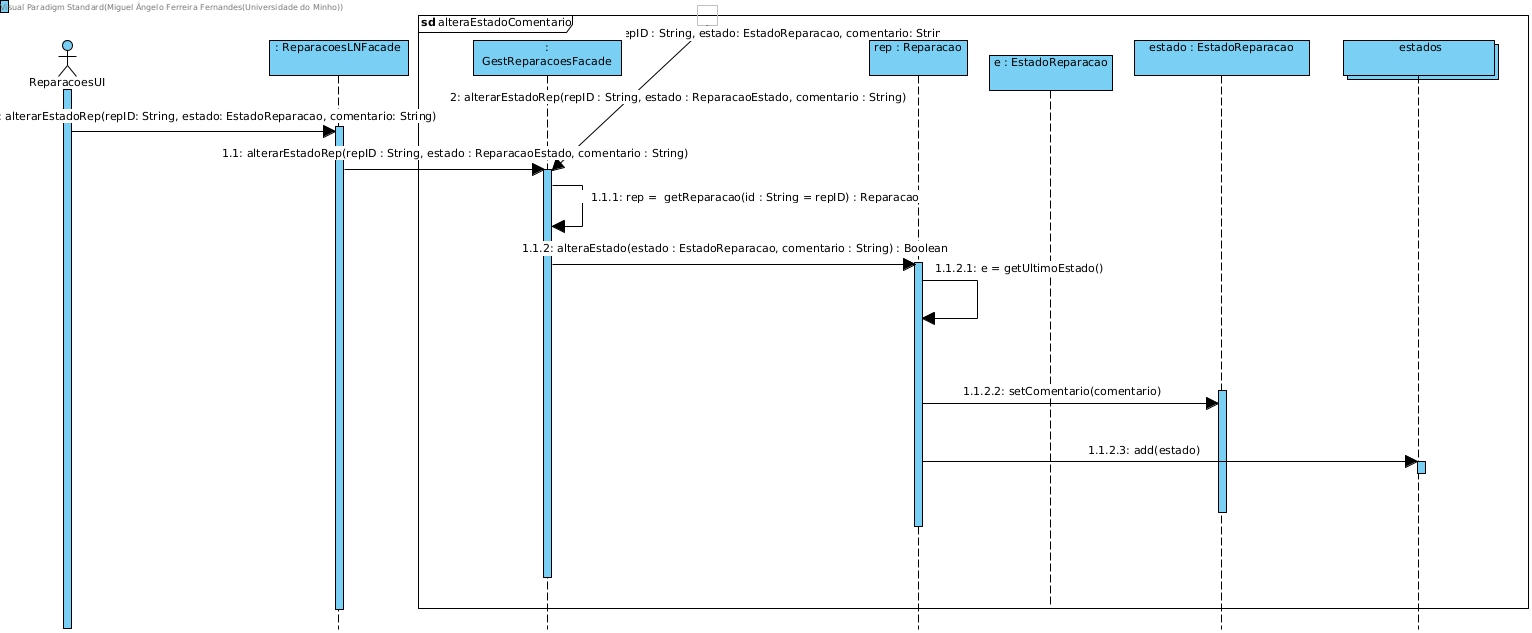
\includegraphics[scale=0.30]{../assets/diagramas_sequencia/sd-AlterarEstadoRep.jpg}
    \caption{Diagrama de sequência AlterarEstadoRep}
\end{figure}

Após o estado mudar, caso se trate de um reparação pogramada o técnico vai realizando, sequencialmente, os passos da reparação do plano de trabalhos,
acrescentando estes aos passos realizados e indicando o tempo gasto e ainda o custo efetivo. Quando não existe mais passos para serem realizados a 
reparação é dada como concluida e o equipamento passa a estar pronto para levantar. No outro caso, em que a reparação é expresso, o técnico limita-se a
registar a conclusão alterando, da mesma forma que a anterior, o estado da reparação e o estado do equipamento.

\begin{figure}[!ht]
    \centering
    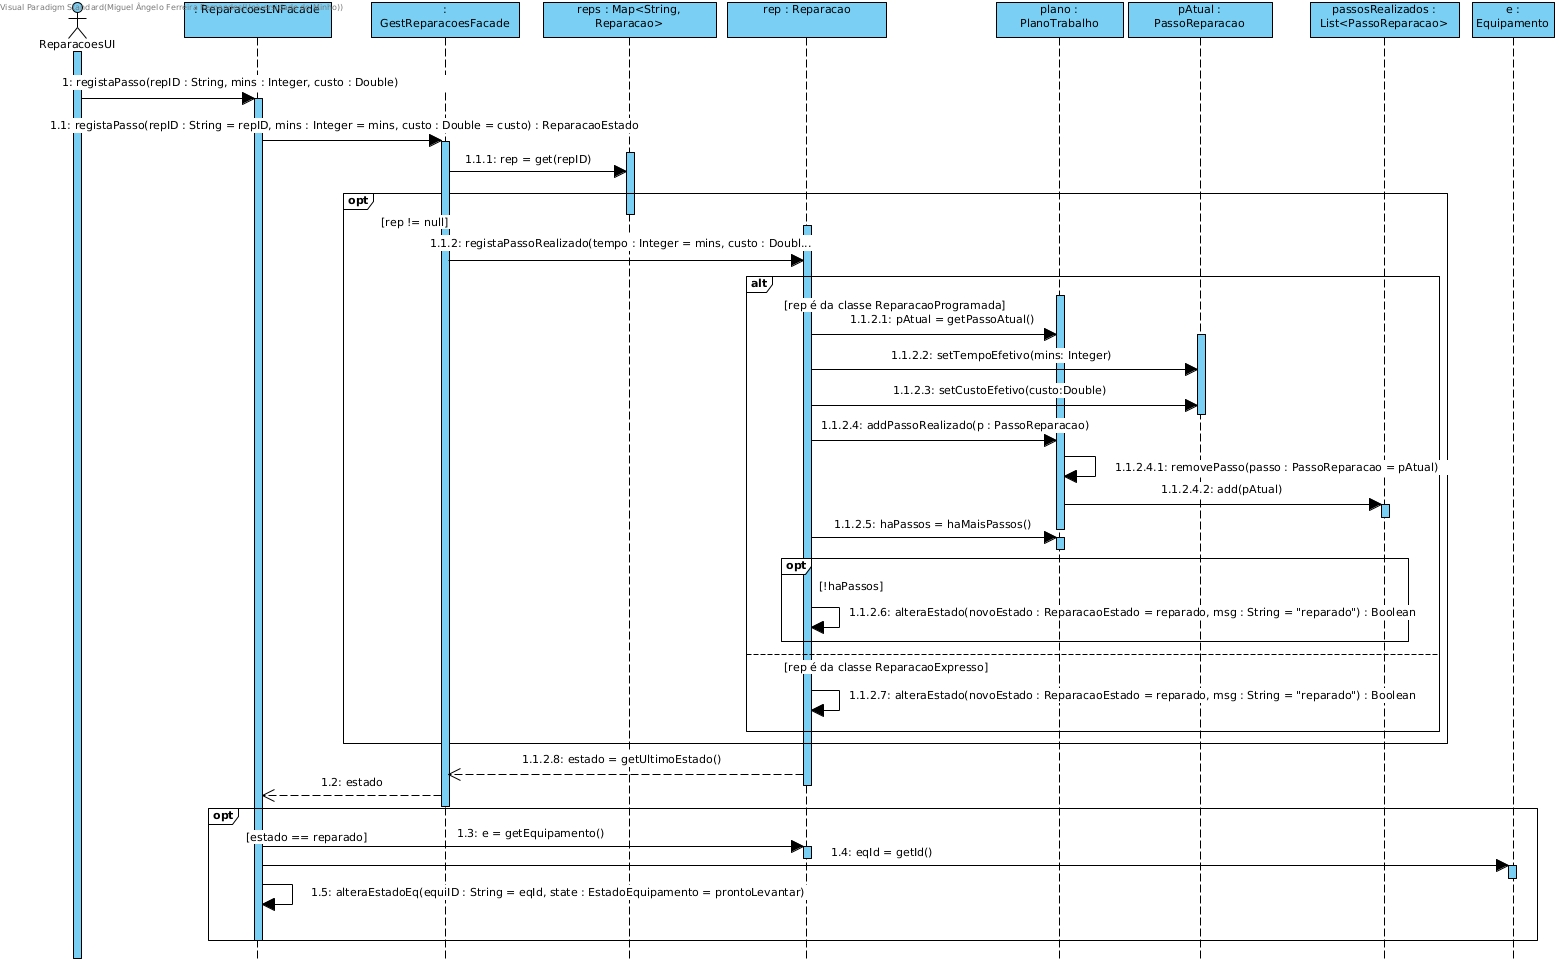
\includegraphics[scale=0.30]{../assets/diagramas_sequencia/sd-RegistaPasso.jpg}
    \caption{Diagrama de sequência registarPasso}
\end{figure}

\subsection{Pedir Reparação Expresso}

O funcionário de balcão é o responsável por realizar os pedidos de reparação expresso. Após identificar o cliente e o equipamento deste, é inserido
no sistema o nome da reparação expresso a ser realizada.
Após a insersão de dados, em primeiro lugar é verificado se o nome corresponde a alguma reparação expresso dísponivel no sistema. Caso esta verificação
seja sucedida, o sistema verifica se existe disponiblidade para realizar a reparação de imediato, isto é, até à hora do fim do centro de reparações.
Para o sistema concluir se existe disponiblidade, este percorre as agendas de todos os técnicos e verifica se existe algum "buraco", onde seja
possível encaixar a reparação pedida. Caso se verifique disponiblidade, é retornado qual o técnico atribuido e a reparação é aceite, caso contrário a
reparação é recusada.
De maneira a que receções de equipamentos por partes dos funcionários de balcão fiquem registadas, é ainda no método addRepExpresso passado o identificador
do funcionário responsável para que seja criada uma instância da classe balcão que será guardada numa lista que mais tarde pode ser analisada pelo gestor.

\begin{figure}[!ht]
    \centering
    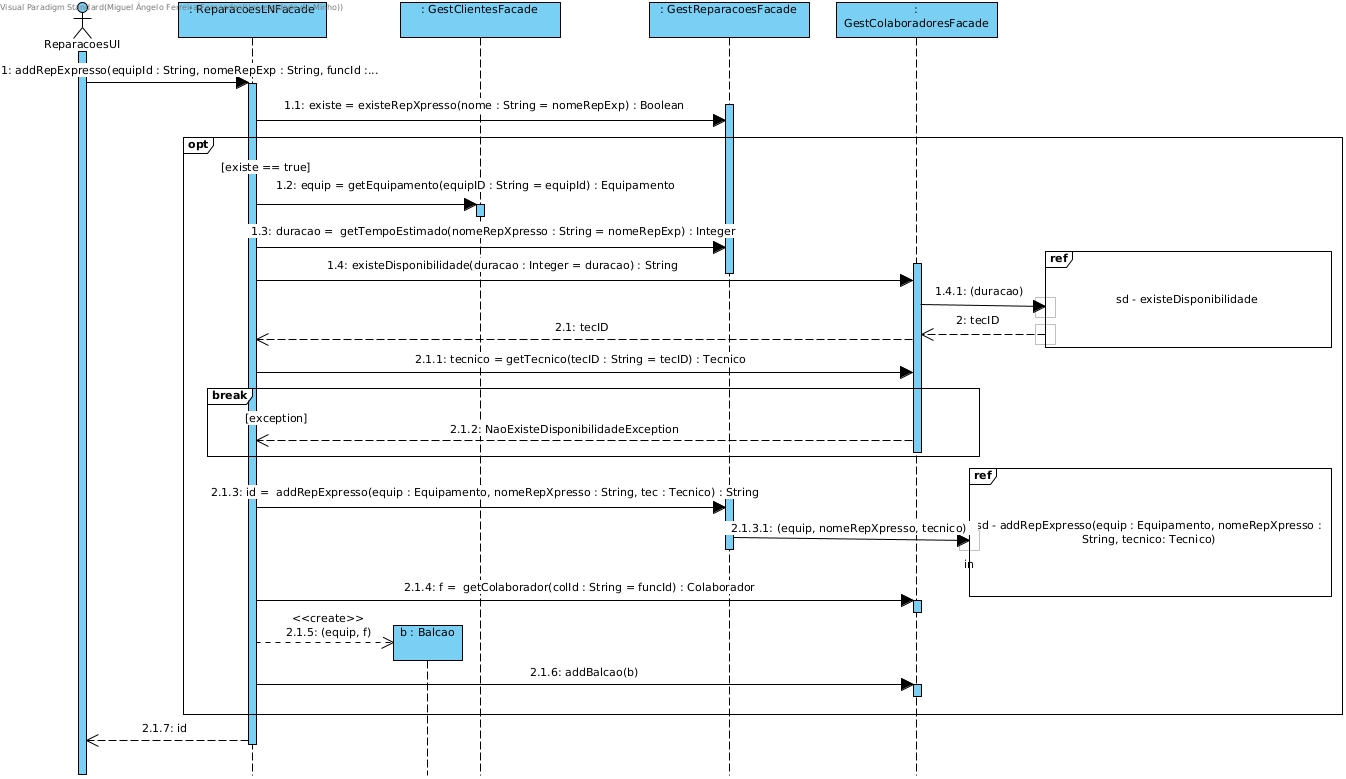
\includegraphics[scale=0.30]{../assets/diagramas_sequencia/sd-addRepExpresso.jpg}
    \caption{Diagrama de sequência addRepExpresso(1)}
\end{figure}

\begin{figure}[!ht]
    \centering
    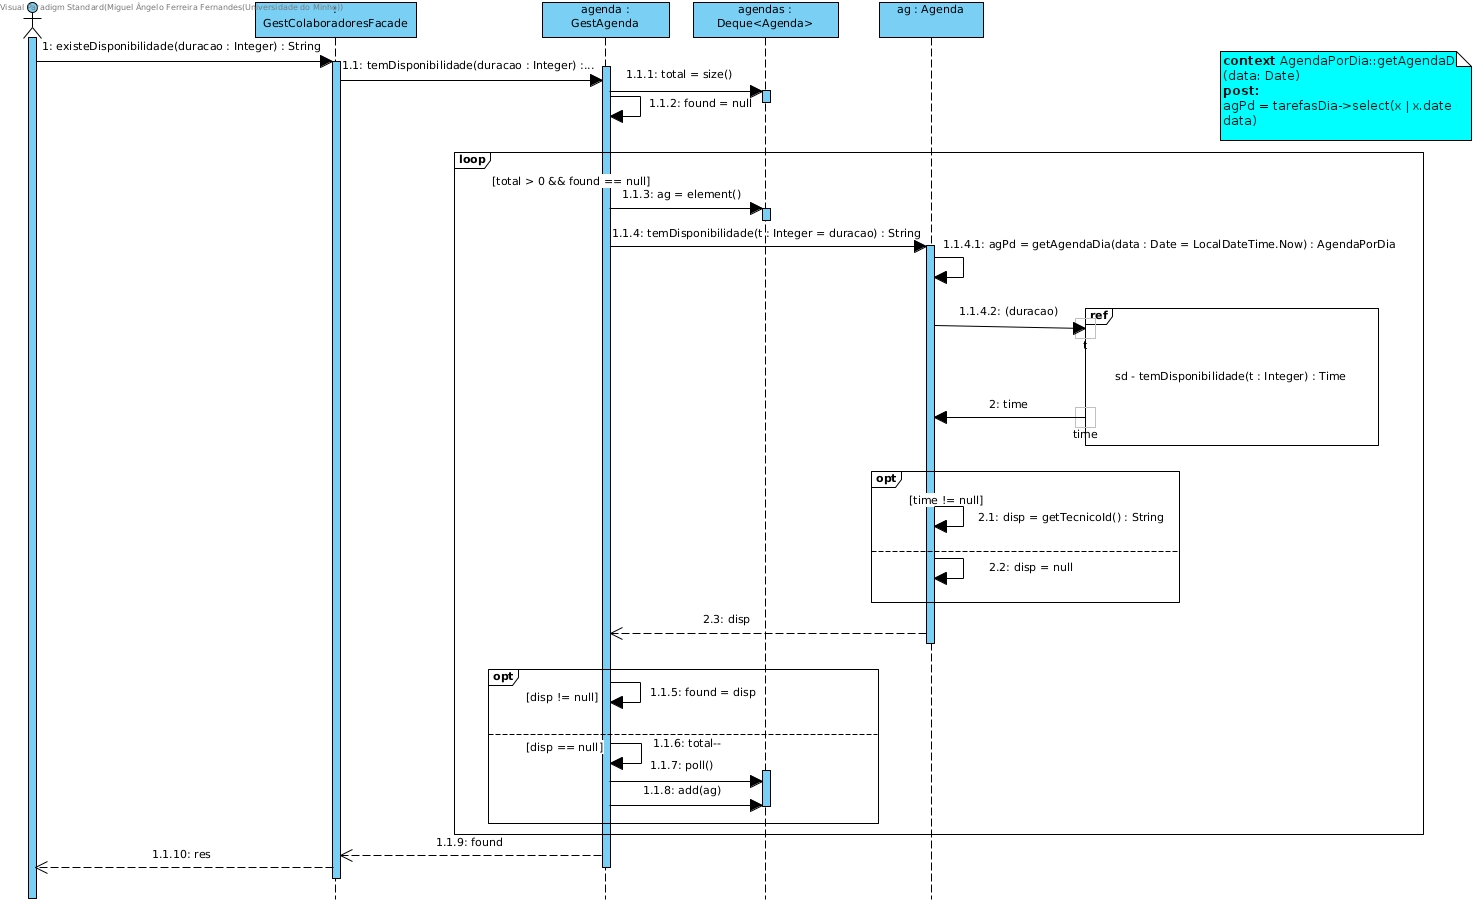
\includegraphics[scale=0.30]{../assets/diagramas_sequencia/sd-existeDisponibilidade.jpg}
    \caption{Diagrama de sequência existeDisponibilidade}
\end{figure}

\begin{figure}[!ht]
    \centering
    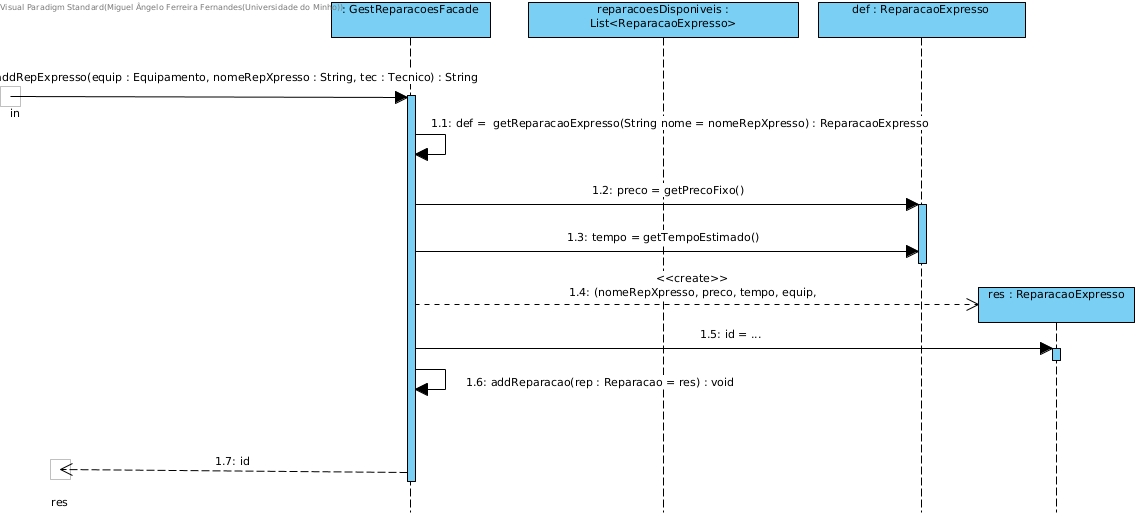
\includegraphics[scale=0.30]{../assets/diagramas_sequencia/sd-addRepExpresso(2).jpg}
    \caption{Diagrama de sequência addRepExpresso(2)}
\end{figure}

\begin{figure}[!ht]
    \centering
    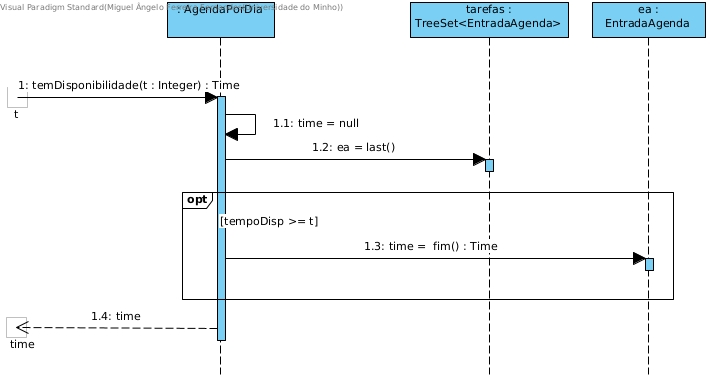
\includegraphics[scale=0.30]{../assets/diagramas_sequencia/sd-temDisponibilidade.jpg}
    \caption{Diagrama de sequência temDisponibilidade}
\end{figure}
    
\end{document}